%\documentclass[options]{class}
\documentclass[10pt,journal]{IEEEtran}
%Paquete de Idioma
\usepackage[english, spanish]{babel}
%Codificación Alfabeto
\usepackage[utf8]{inputenc}
%Codificación de Fuente
\usepackage[T1]{fontenc}
%Índice
\usepackage{makeidx}
%Gráficos
\usepackage{graphicx}
\usepackage{float} 
%Matemáticas
\usepackage{amsmath}
\usepackage{amsfonts}
\usepackage{amssymb}
%Paquetes varios
\usepackage{fullpage}
\usepackage{apacite}
\usepackage{lipsum}
\usepackage{pdfpages}
\usepackage{upgreek}
\usepackage{float}
\usepackage{latexsym}
\usepackage{url}
\usepackage{adjustbox}
\usepackage{gensymb}
\usepackage{multicol}
\usepackage{mathtools, nccmath}
\usepackage{caption}
\usepackage{subcaption}
\usepackage{multirow}
\usepackage{enumerate}
\usepackage{array,tabularx}
\usepackage{cleveref}
%Hiperlinks \href{url}{text}
\usepackage[pdftex]{hyperref}
\begin{document}

%Título
\title{\textbf{Práctica 1.} Interacciones entre la materia: La carga eléctrica}
%Autor
\author{Universidad Nacional Autónoma de México, Facultad de Ciencias\\ Laboratorio de Electromagnetismo\\
Aguirre Pérez Alexander\\ Barranco Peña Israel Daniel\\  Hernandez Azuz Adán\\ López Merino Marcos\\ Wada Reyes Oscar\\ \today }
\maketitle{}  
%Resumen
\begin{abstract}
En este trabajo se cargaron eléctricamente barras de distintos materiales (cobre, aluminio, vidrio, PVC, etc) cuando se frotaban con piel animal, hule espuma y diferentes telas; usando un electroscopio se determinó el signo de la carga obtenida en los materiales (positiva o negativa) y se estimó la cantidad de
carga presente en las barras media. A su vez, también se provocó el exceso de carga en las distintas barras mediante el frotamiento y hasta obtener el ángulo máximo de inclinación provocado por cada barra en la aguja del electroscopio para después descargar eléctricamente las barras mediante el contacto con un material eléctricamente neutro.
\end{abstract}
%%%%%%%%%%%%%%%%%%%%%%%%%%%%%%%%%%%%%%%%
\section{Objetivos}
En este trabajo se propusieron los siguientes objetivos:
\begin{itemize}
    \item Definir el concepto de carga eléctrica.
    \item Determinar los distintos tipos de carga que puede obtener la materia.
    \item Provocar el exceso de carga en distintos materiales.
    \item Descargar los diferentes materiales mediante distintos métodos.
\end{itemize}
%%%%%%%%%%%%%%%%%%%%%%%%%%%%%%%%%%%%%%%%%%%%%
\section{Marco Teórico}
La neutralidad eléctrica de la mayoría de los objetos en nuestro mundo visible y tangible oculta el contenido de cantidades enormes de carga eléctrica positiva y negativa que, en su mayor parte, se cancelan entre si en sus efectos externos \cite{resnick2002fisica}. Sólo cuando este equilibrio eléctrico se perturba, la naturaleza nos revela los efectos de una carga positiva o negativa no compensada. Cuando decimos que un objeto está «cargado» queremos decir que tiene un desbalance de carga, aún cuando la carga neta represente generalmente tan solo una pequeñísima fracción de la carga positiva o negativa total contenida en el cuerpo \cite{barco2012fisica}. El tipo de carga (positiva o negativa) se asigna de manera convencional. Los objetos cargados ejercen fuerzas entre sí. Consideremos dos pequeñas esferas de ebonita (caucho vulcanizado con azufre) que han sido previamente frotadas con piel, y que luego se cuelgan mediante hilos de seda como se muestra en la Figura \ref{Fig: Fuerzas_unidas}.(\subref{Fig: Fuerzas_b}); se observa que las dos esferas se repelen.\\
Seguidamente consideremos dos esferas pequeñas de vidrio que han
sido previamente frotadas con seda, colgadas mediante hilos de seda como se muestra en la Figura \ref{Fig: Fuerzas_unidas}.(\subref{Fig: Fuerzas_b}); se observa que las dos esferas también se repelen.\\
Ahora, si se cuelgan mediante hilos de seda una esfera de ebonita y una esfera de vidrio como se muestra en la Figura \ref{Fig: Fuerzas_unidas}.(\subref{Fig: Fuerzas_a}), se observará que las dos esferas se atraen.\\
En general, si dos cuerpos diferentes se frotan entre sí, ambos se electrizan, es decir, ambos se cargan eléctricamente.\\ 
\begin{figure*}
\centering
\begin{subfigure}{.4\textwidth}
\includegraphics[width = .5\linewidth]{Figuras/fuerzaatraccion.PNG}
\caption{}
\label{Fig: Fuerzas_a}
\end{subfigure}%
\centering
\begin{subfigure}{.4\textwidth}
\includegraphics[width = .5\linewidth]{Figuras/fuerzarepulsion.PNG}
\caption{}
\label{Fig: Fuerzas_b}
\end{subfigure}
\caption{Fuerzas eléctricas: (\subref{Fig: Fuerzas_a}) Muestra lo que sucede cuando hay fuerzas de atracción y (\subref{Fig: Fuerzas_b}) Muestra lo que sucede cuando hay fuerzas repulsivas}
\label{Fig: Fuerzas_unidas}
\end{figure*}
%%%%%%%%%%%%%%%%%%%%%%%%%%%%%%%%%%%%%%%%%%%%%%5
\section{Diseño Experimental}
%---------------------------------------------------
\subsection{Montaje experimental}
\begin{figure}
\begin{flushleft}
\includegraphics[scale=0.3]{Figuras/Montaje_experimental.png}
\caption{Montaje experimental con el cual se obtuvieron las mediciones correspondientes al experimento.}
\label{Fig: Montaje}
\end{flushleft}
\end{figure}
Para el montaje experimental, primero se pegó con cinta adhesiva el transportador a la parte trasera del electroscopio y detrás de éste se colocó una hoja cuadriculada que sirviera como referencia para la determinación de los ángulos para cada una de las mediciones realizadas. Se utilizó un nivel ojo de buey para determinar la inclinación del espacio de trabajo, debido a que una inclinación muy pronunciada perjudicaría las mediciones realizadas. Dado que se observó una inclinación apreciable, se procedió a nivelar todo el montaje experimental que se tenía hasta ese momento.\\
Después, se colocó una varilla con una nuez ajustada a un extremo y otra que la ajustaba al soporte a una cierta distancia del piso\footnote{La distancia en la que se encontraba la varilla en el soporte dependía de la longitud de cada una de las barras de metal utilizadas.}; donde el soporte con la varilla se colocó detrás del electroscopio. Asimismo, se colocó una «protuberancia» en cada una de las barras, de las manera que la distancia entre éstas y la esfera metálica del electroscopio fuese de $0.5cm \pm 0.05 cm$.(\textit{Véase} 
Figura \ref{Fig: Distancia})\\
\begin{figure}
\begin{center}
\includegraphics[scale=0.3]{Figuras/distancia_1.png} 
\end{center}
\caption{Acercamiento del montaje que nos muestra la distancia que debe haber entre la barra y la esfera metálica, donde $d = 0.5cm \pm 0.05 cm$.}
\label{Fig: Distancia}
\end{figure}
Finalmente, frente al electroscopio se colocó la varilla que sostenía al teléfono en soporte restante ajustada con una nuez a éste. (\textit{Véase} Figura \ref{Fig: Montaje})
%-------------------------------------------------
\subsection{Proceso experimental}
Antes de comenzar con las mediciones correspondientes, se hizo una calibración del electroscopio proporcionándole un cierto voltaje con la fuente de alimentación (i.e. conectando la fuente de alimentación directamente al electroscopio) entre $2kV$ y $5kV$, lo cual permitió encontrar un intervalo, i.e. encontrar un valor máximo y uno mínimo del ángulo $\theta$.(\textit{Véase} Figura \ref{Fig: Angles})\\
\begin{figure}
\centering
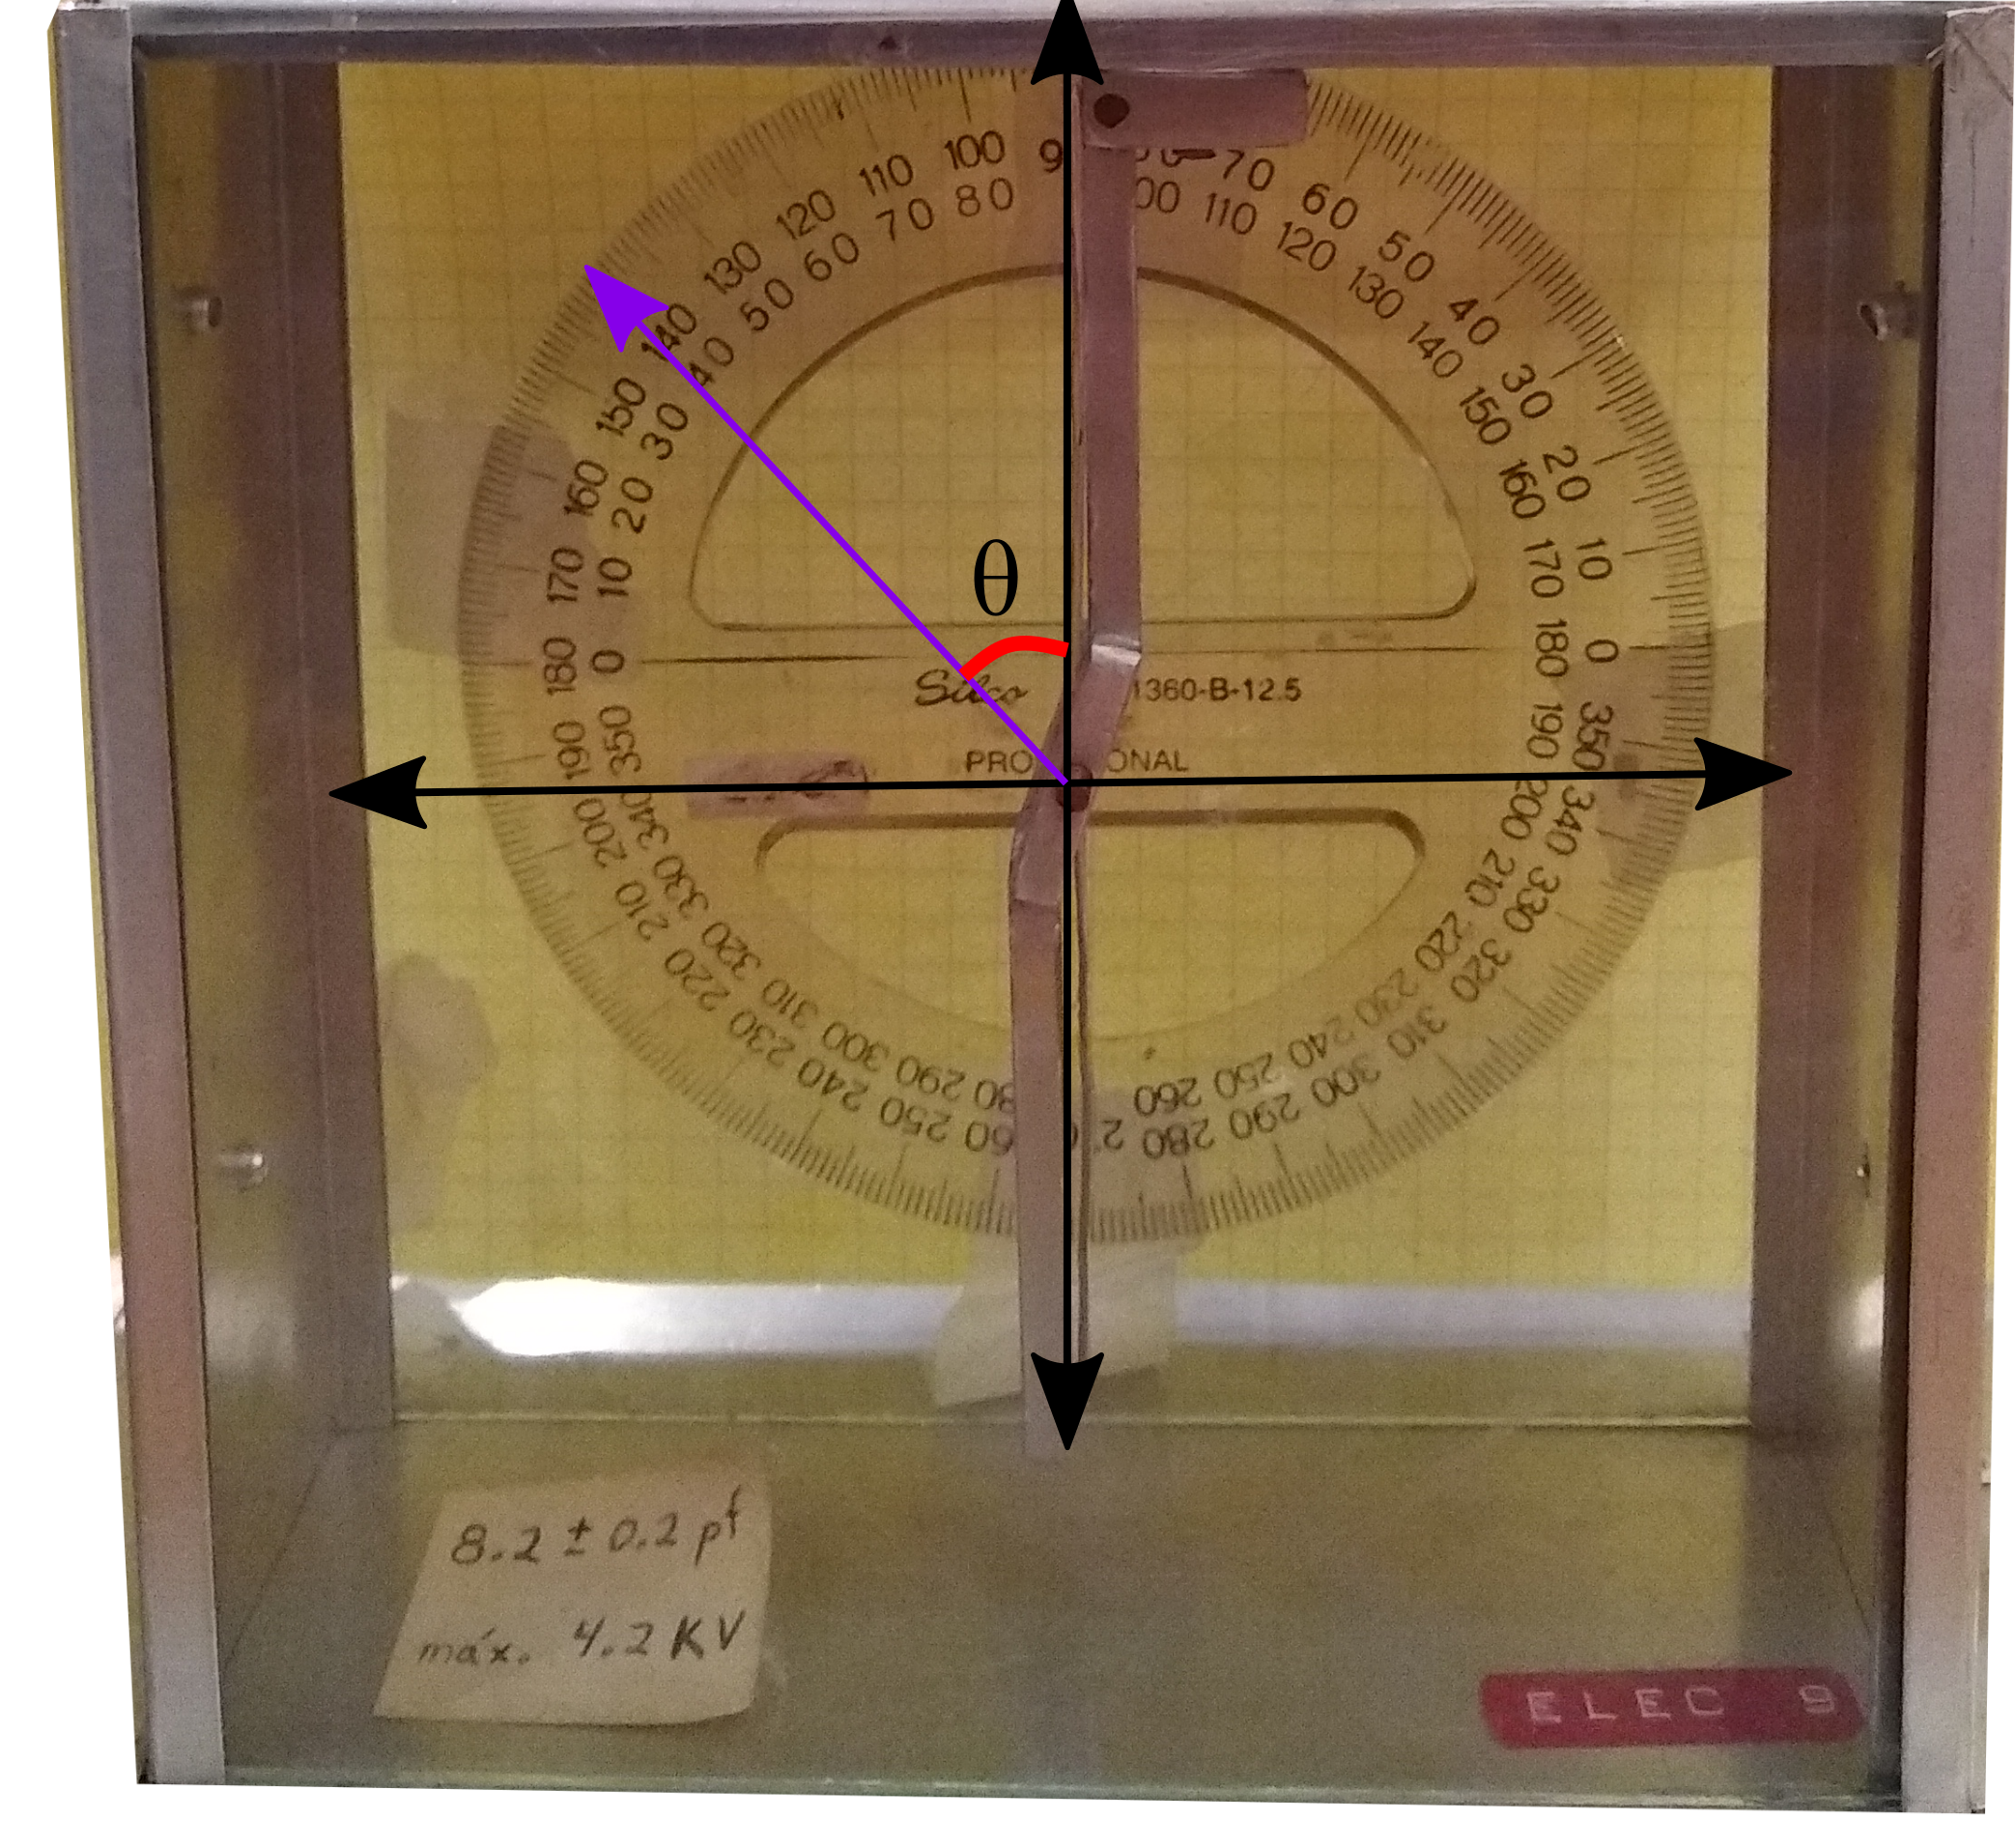
\includegraphics[scale=0.08]{Figuras/angles_1.png} 
\caption{Representación gráfica de los ejes de referencia y la manera en que fue medida el ángulo}
\label{Fig: Angles}
\end{figure}
Posteriormente, con las diferentes telas\footnote{Terciopelo, hule espuma, piel y elastano.} se procedió a cargar eléctricamente, por medio de la fricción, cada una de las barras\footnote{Barra de vidrio, acrílico y PVC.} con las telas disponibles. Una vez \textit{cargada} la barra, se colocaba en la nuez disponible sobre el electroscopio y, al mismo tiempo, se capturó un vídeo (o una fotografía) del ángulo generado al acercar la barra; esto se repitió para cada una de las barras.\\
Finalmente, para tener una relación entre los ángulos obtenidos y el voltaje, se conectó la fuente de alimentación al electroscopio. Es decir, se le proporcionaron diferentes voltajes (0.8 $kV$ a 5.0$kV$) y se capturó la inclinación de la varilla contenida dentro del electroscopio. Por último, se hizo el análisis correspondientes de los datos obtenidos.
%%%%%%%%%%%%%%%%%%%%%%%%%%%%%%%%%%%%%%%%%%%%%%%%%
\section{Resultados}

Carga del electroscopio:
\begin{equation*}
    C = (8.2 \pm 0.2)pf
\end{equation*}


\begin{figure}[H]
\centering
\includegraphics[scale=0.25]{tablasignos.png}
\caption{Registro de los ángulos observados ($^{o}$) en el electroscopio, con cada varilla para cada una de las telas, así como el tipo de carga asociado a cada medición.}
\end{figure}

\begin{figure}[H]
\centering
\includegraphics[scale=0.35]{tablapotencial.png}
\caption{Registro de los ángulos generados en el electroscopio, a partir de distintos potenciales eléctricos provenientes de una fuente eléctrica.}
\end{figure}

\begin{figure}[H]
\centering
\includegraphics[scale=0.35]{grafpot.png}
\caption{Gráfica  de  los  datos  experimentales  de  potencial eléctrico y ángulo, a  partir  de los datos de la figura 6, así como el ajuste polinomial a la curva (color azul).}
\label{Fig: Datos}
\end{figure}

En la Figura \ref{Fig: Datos}, se observa la curva obtenida a partir la variación de potencial eléctrico a través de un electroscopio que va relacionado con el ángulo generado entre las placas metálicas del electroscopio. Los marcadores color negro corresponden a cada medición realizada, así como la incertidumbre asociada a la fuente eléctrica y el transportador utilizado (barras rojas).\\

En este sentido, la cantidad de potencial eléctrico medido está asociado a la carga generada por fricción entre las varillas y cada tipo de tela empleada.

\begin{figure}[H]
\centering
\includegraphics[scale=0.3]{piel.png}
\caption{Registro del cálculo del potencial eléctrico asociado a la carga generada por fricción entre cada varilla y piel, a partir de la ecuación obtenida del ajuste polinomial de la figura \ref{Fig: Datos}.}
\end{figure}

\begin{figure}[H]
\centering
\includegraphics[scale=0.29]{terciopelo.png}
\caption{Registro del cálculo del potencial eléctrico asociado a la carga generada por fricción entre cada varilla y terciopelo, a partir de la ecuación obtenida del ajuste polinomial de la figura \ref{Fig: Datos}.}
\end{figure}

\begin{figure}[H]
\centering
\includegraphics[scale=0.30]{huleespuma.png}
\caption{Registro del cálculo del potencial eléctrico asociado a la carga generada por fricción entre cada varilla y hule espuma, a partir de la ecuación obtenida del ajuste polinomial de la figura \ref{Fig: Datos}.}
\end{figure}

\begin{figure}[H]
\centering
\includegraphics[scale=0.30]{elastano.png}
\caption{Registro del cálculo del potencial eléctrico asociado a la carga generada por fricción entre cada varilla y elastano, a partir de la ecuación obtenida del ajuste polinomial de la figura \ref{Fig: Datos}.}
\end{figure}

Los errores mostrados en las figuras 8, 9, 10 y 11, se calcularon a partir de la derivación de la ecuación del ajuste polinomial, de tal manera que:

\begin{equation*}
    \delta V = |2*0.0006*\theta -0.0018|*\delta\theta
\end{equation*}


El error relativo porcentual estuvo dado por:

\begin{equation*}
    \delta E = \frac{\delta V}{V}*100
\end{equation*}\\

%%%%%%%%%%%%%%%%%%%%%%%%%%%%%%%%%%%%%%%%%%%%%%%%%%%
\section{Discusión de Resultados}
A partir de las mediciones realizadas y el análisis de estos datos se obtiene en primer lugar un importante resultado de la naturaleza de las cargas, y es que esta puede ser o negativa o positiva; esto es fácil de apreciar al analizar la "Figura 5.", ya que el alambre del electroscopio podía o alejarse o acercarse a la varilla, lo que nos indicaba los diferentes signos de los materiales cargados.
Continuando con el análisis de estos datos, a partir de la gráfica resultante del ajuste polinomial mostrado en la "Figura 7.", se encuentra igualmente la relación entre las mediciones del electroscopio y las diferencias de potencial eléctrico generadas por la carga inducida por el material, y se observa claramente que al variar el material estas cargas van a cambiar, ya que al tener la misma distancia, la variable que afecta el valor del potencial eléctrico es la carga del material.
Aunque estos resultados son meramente cualitativos, nos hablan de importantes propiedades de la carga y nos dan una fuerte introducción a la manera en la que un objeto puede cargarse (por inducción en este caso), de cómo la carga inducida depende del signo de la carga original y nos enseña que al descargar un cuerpo, cualquier comportamiento ocasionado por esta carga, desaparecerá.
%%%%%%%%%%%%%%%%%%%%%%%%%%%%%%%%%%%%%%%%%%%%%%
\section{Conclusiones}
Durante el experimento se logró comprobar la existencia de 2 tipos distintos de carga presentes debido a la transferencia de electrones de un material a otro.\\
Se comprobó la existencia de dos cargas presentes, observando la respuesta que se producía en el electroscopio  al acercarle una barra frotada previamente con cierta tela o material.
La barra móvil del electroscopio giraba formando un ángulo respecto a la varilla vertical, este hecho nos permitió observar que se hacía presente una fuerza que lograba que la barra móvil se mantuviera en equilibrio. Esto debido a que la barra móvil había adquirido cierta carga contraria a la varilla fija.\\
La existencia de la otra carga se estableció cuando al electroscopio previamente cargado, es decir cuándo  la varilla móvil formarse un ángulo con la vertical y se mantuviera en equilibrio, se le acercó una de las barras frotada con un distinto material (tela), esto provocó que la varilla móvil del electroscopio regresará a su posición original de reposo.\\
Con esto comprobamos que existen 2 tipos de cargas existentes en la naturaleza que provocan fuerzas de repulsión o de atracción. La fuerza de repulsión se presenta cuando dos cargas de la misma naturaleza se acercan y la de atracción cuando dos cargas distintas se encuentran.\\
Además, con los datos obtenidos verificamos que la relación entre la fuerza presente debido a la atracción o repulsión de las cargas y la distancia entre ellas varía de manera inversamente proporcional. Ya que a una distancia mayor entre la barra que previamente había adquirido una carga debido al frotamiento y la esfera del electroscopio, el ángulo presente era menor en comparación a aquel que se presentaba cuando existía una separación más pequeña.
Durante el desarrollo experimentan empleamos los distintos métodos de electrificación.\\
Por frotamiento: cada vez que frotábamos las barras con las diferentes fibras, cada material cedía o adquiría electrones provocando una diferencia en su carga original.\\
Por Inducción:  Acercamos un objeto cargado eléctricamente (barra) a un cuerpo conductor neutro, en este caso la esfera del electroscopio, sin establecer contacto físico con él provocando que los electrones del conductor se redistribuyeran. Así  cumplimos los objetivos trazados al inicio de la practica, verificando la existencia de los tipos de cargas y clasificándolas, además de deducir la la relación de proporcionalidad entre la fuerza y la distancia provocado por la interacción de las cargas, también relacionamos los ángulos obtenidos con el voltaje presente durante el proceso de electrificación que ocurría en el electroscopio.
Por lo que los conceptos adquiridos nos permitieron entender las bases de la electrostática y entender el origen del electromagnetismo.
%%%%%%%%%%%%%%%%%%%%%%%%%%%%
\bibliographystyle{apacite}
\bibliography{referencias}
\end{document}







